\documentclass{standalone}
\usepackage{tikz}
\usetikzlibrary{patterns, positioning}


\begin{document}
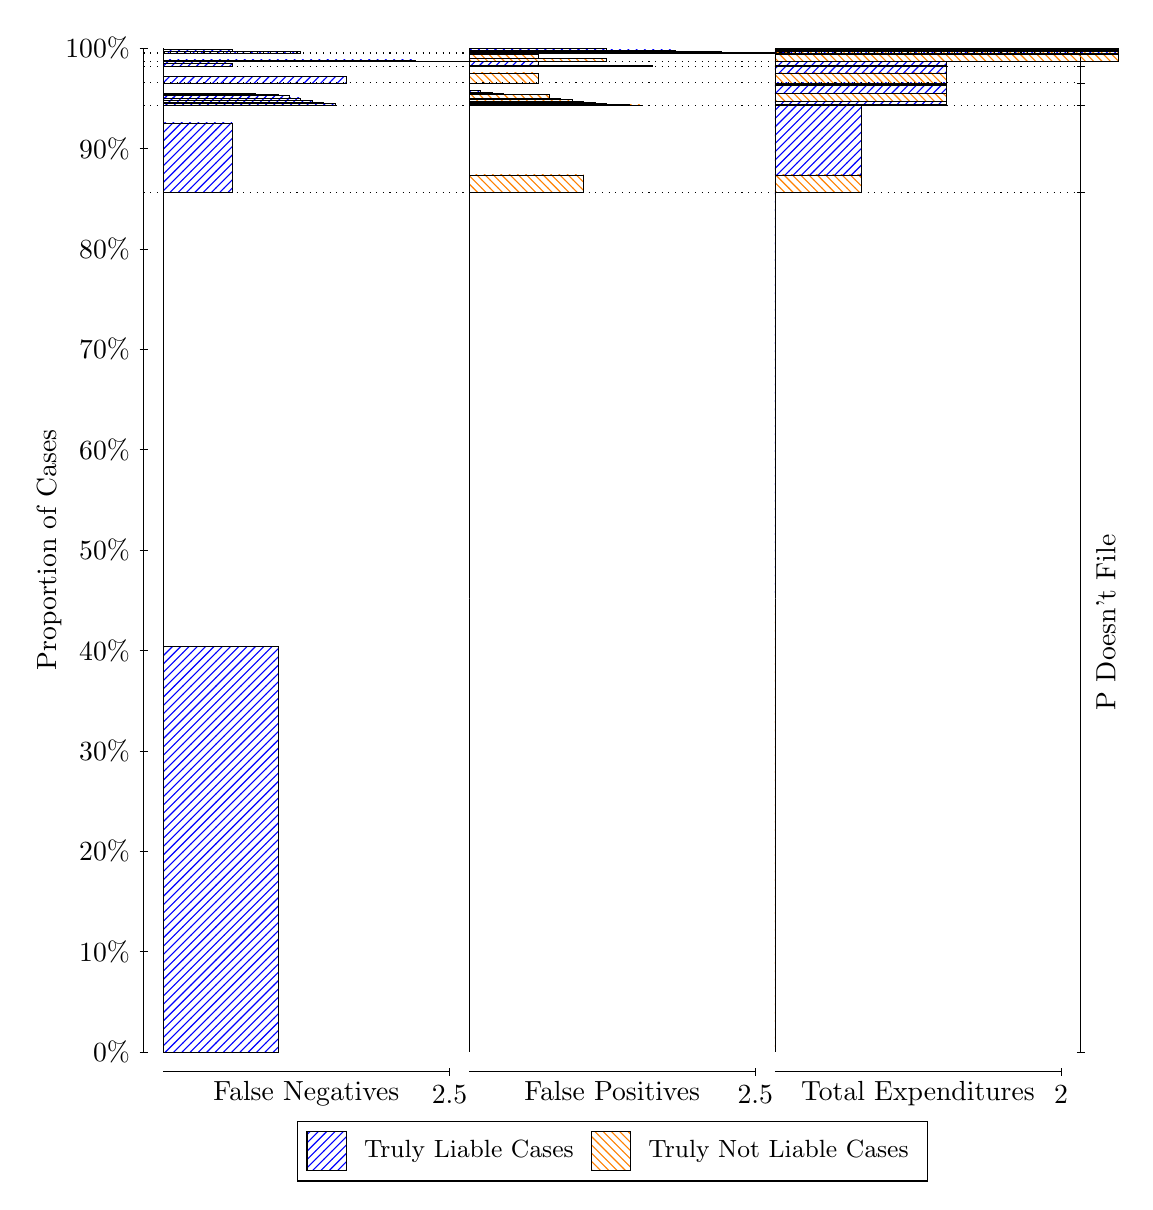
\begin{tikzpicture}
\draw[black, very thin] (1.5,1.75) -- (1.5,14.5);
\node[rotate=90, text=black, anchor=center] at (0.3, 8.125) {Proportion of Cases};
\draw[black, very thin] (1.45,1.75) -- (1.55,1.75);
\node[text=black, anchor=east] at (1.45, 1.75) {0\%};
\draw[black, very thin] (1.45,3.025) -- (1.55,3.025);
\node[text=black, anchor=east] at (1.45, 3.025) {10\%};
\draw[black, very thin] (1.45,4.3) -- (1.55,4.3);
\node[text=black, anchor=east] at (1.45, 4.3) {20\%};
\draw[black, very thin] (1.45,5.575) -- (1.55,5.575);
\node[text=black, anchor=east] at (1.45, 5.575) {30\%};
\draw[black, very thin] (1.45,6.85) -- (1.55,6.85);
\node[text=black, anchor=east] at (1.45, 6.85) {40\%};
\draw[black, very thin] (1.45,8.125) -- (1.55,8.125);
\node[text=black, anchor=east] at (1.45, 8.125) {50\%};
\draw[black, very thin] (1.45,9.4) -- (1.55,9.4);
\node[text=black, anchor=east] at (1.45, 9.4) {60\%};
\draw[black, very thin] (1.45,10.675) -- (1.55,10.675);
\node[text=black, anchor=east] at (1.45, 10.675) {70\%};
\draw[black, very thin] (1.45,11.95) -- (1.55,11.95);
\node[text=black, anchor=east] at (1.45, 11.95) {80\%};
\draw[black, very thin] (1.45,13.225) -- (1.55,13.225);
\node[text=black, anchor=east] at (1.45, 13.225) {90\%};
\draw[black, very thin] (1.45,14.5) -- (1.55,14.5);
\node[text=black, anchor=east] at (1.45, 14.5) {100\%};

\draw[black, very thin] (13.4,1.75) -- (13.4,14.5);
\draw[black, very thin] (13.35,1.75) -- (13.45,1.75);
\node[anchor=west] at (13.35, 1.75) {};
\draw[black, very thin] (13.35,12.664) -- (13.45,12.664);
\node[anchor=west] at (13.35, 12.664) {};
\draw[black, very thin] (13.35,13.774) -- (13.45,13.774);
\node[anchor=west] at (13.35, 13.774) {};
\draw[black, very thin] (13.35,14.058) -- (13.45,14.058);
\node[anchor=west] at (13.35, 14.058) {};
\draw[black, very thin] (13.35,14.265) -- (13.45,14.265);
\node[anchor=west] at (13.35, 14.265) {};
\draw[black, very thin] (13.35,14.327) -- (13.45,14.327);
\node[anchor=west] at (13.35, 14.327) {};
\draw[black, very thin] (13.35,14.437) -- (13.45,14.437);
\node[anchor=west] at (13.35, 14.437) {};
\draw[black, very thin] (13.35,14.5) -- (13.45,14.5);
\node[anchor=west] at (13.35, 14.5) {};

\draw[black, very thin, pattern color=blue, pattern=north east lines] (1.75,1.75) rectangle (3.2033,6.9023);
\draw[black, very thin, pattern color=orange, pattern=north west lines] (1.75,6.9023) rectangle (1.75,12.664);
\draw[black, very thin, pattern color=blue, pattern=north east lines] (1.75,12.664) rectangle (2.622,13.548);
\draw[black, very thin, pattern color=orange, pattern=north west lines] (1.75,13.548) rectangle (1.75,13.774);
\draw[black, very thin, pattern color=blue, pattern=north east lines] (1.75,13.774) rectangle (3.93,13.798);
\draw[black, very thin, pattern color=blue, pattern=north east lines] (1.75,13.798) rectangle (3.7847,13.806);
\draw[black, very thin, pattern color=blue, pattern=north east lines] (1.75,13.806) rectangle (3.6393,13.835);
\draw[black, very thin, pattern color=blue, pattern=north east lines] (1.75,13.835) rectangle (3.494,13.867);
\draw[black, very thin, pattern color=blue, pattern=north east lines] (1.75,13.867) rectangle (3.3487,13.898);
\draw[black, very thin, pattern color=blue, pattern=north east lines] (1.75,13.898) rectangle (3.2033,13.908);
\draw[black, very thin, pattern color=blue, pattern=north east lines] (1.75,13.908) rectangle (3.058,13.916);
\draw[black, very thin, pattern color=blue, pattern=north east lines] (1.75,13.916) rectangle (2.9127,13.921);
\draw[black, very thin, pattern color=blue, pattern=north east lines] (1.75,13.921) rectangle (2.7673,13.925);
\draw[black, very thin, pattern color=orange, pattern=north west lines] (1.75,13.925) rectangle (1.75,14.058);
\draw[black, very thin, pattern color=blue, pattern=north east lines] (1.75,14.058) rectangle (4.0753,14.138);
\draw[black, very thin, pattern color=orange, pattern=north west lines] (1.75,14.138) rectangle (1.75,14.265);
\draw[black, very thin, pattern color=blue, pattern=north east lines] (1.75,14.265) rectangle (2.622,14.31);
\draw[black, very thin, pattern color=orange, pattern=north west lines] (1.75,14.31) rectangle (1.75,14.327);
\draw[black, very thin, pattern color=blue, pattern=north east lines] (1.75,14.327) rectangle (5.8193,14.333);
\draw[black, very thin, pattern color=blue, pattern=north east lines] (1.75,14.333) rectangle (4.9473,14.349);
\draw[black, very thin, pattern color=orange, pattern=north west lines] (1.75,14.349) rectangle (1.75,14.437);
\draw[black, very thin, pattern color=blue, pattern=north east lines] (1.75,14.437) rectangle (3.494,14.46);
\draw[black, very thin, pattern color=blue, pattern=north east lines] (1.75,14.46) rectangle (2.622,14.479);
\draw[black, very thin, pattern color=orange, pattern=north west lines] (1.75,14.479) rectangle (1.75,14.5);
\draw[black, very thin, pattern color=orange, pattern=north west lines] (5.6333,1.75) rectangle (5.6333,7.5121);
\draw[black, very thin, pattern color=blue, pattern=north east lines] (5.6333,7.5121) rectangle (5.6333,12.664);
\draw[black, very thin, pattern color=orange, pattern=north west lines] (5.6333,12.664) rectangle (7.0867,12.89);
\draw[black, very thin, pattern color=blue, pattern=north east lines] (5.6333,12.89) rectangle (5.6333,13.774);
\draw[black, very thin, pattern color=orange, pattern=north west lines] (5.6333,13.774) rectangle (7.8133,13.778);
\draw[black, very thin, pattern color=orange, pattern=north west lines] (5.6333,13.778) rectangle (7.668,13.781);
\draw[black, very thin, pattern color=orange, pattern=north west lines] (5.6333,13.781) rectangle (7.5227,13.789);
\draw[black, very thin, pattern color=orange, pattern=north west lines] (5.6333,13.789) rectangle (7.3773,13.798);
\draw[black, very thin, pattern color=orange, pattern=north west lines] (5.6333,13.798) rectangle (7.232,13.812);
\draw[black, very thin, pattern color=orange, pattern=north west lines] (5.6333,13.812) rectangle (7.0867,13.823);
\draw[black, very thin, pattern color=orange, pattern=north west lines] (5.6333,13.823) rectangle (6.9413,13.847);
\draw[black, very thin, pattern color=orange, pattern=north west lines] (5.6333,13.847) rectangle (6.796,13.862);
\draw[black, very thin, pattern color=orange, pattern=north west lines] (5.6333,13.862) rectangle (6.6507,13.907);
\draw[black, very thin, pattern color=blue, pattern=north east lines] (5.6333,13.907) rectangle (6.36,13.911);
\draw[black, very thin, pattern color=blue, pattern=north east lines] (5.6333,13.911) rectangle (6.2147,13.916);
\draw[black, very thin, pattern color=blue, pattern=north east lines] (5.6333,13.916) rectangle (6.0693,13.924);
\draw[black, very thin, pattern color=blue, pattern=north east lines] (5.6333,13.924) rectangle (5.924,13.934);
\draw[black, very thin, pattern color=blue, pattern=north east lines] (5.6333,13.934) rectangle (5.7787,13.965);
\draw[black, very thin, pattern color=blue, pattern=north east lines] (5.6333,13.965) rectangle (5.6333,14.058);
\draw[black, very thin, pattern color=orange, pattern=north west lines] (5.6333,14.058) rectangle (6.5053,14.185);
\draw[black, very thin, pattern color=blue, pattern=north east lines] (5.6333,14.185) rectangle (5.6333,14.265);
\draw[black, very thin, pattern color=orange, pattern=north west lines] (5.6333,14.265) rectangle (7.9587,14.283);
\draw[black, very thin, pattern color=blue, pattern=north east lines] (5.6333,14.283) rectangle (6.5053,14.327);
\draw[black, very thin, pattern color=orange, pattern=north west lines] (5.6333,14.327) rectangle (7.3773,14.367);
\draw[black, very thin, pattern color=orange, pattern=north west lines] (5.6333,14.367) rectangle (6.5053,14.416);
\draw[black, very thin, pattern color=blue, pattern=north east lines] (5.6333,14.416) rectangle (5.924,14.431);
\draw[black, very thin, pattern color=blue, pattern=north east lines] (5.6333,14.431) rectangle (5.6333,14.437);
\draw[black, very thin, pattern color=orange, pattern=north west lines] (5.6333,14.437) rectangle (9.7027,14.441);
\draw[black, very thin, pattern color=orange, pattern=north west lines] (5.6333,14.441) rectangle (8.8307,14.458);
\draw[black, very thin, pattern color=blue, pattern=north east lines] (5.6333,14.458) rectangle (8.2493,14.477);
\draw[black, very thin, pattern color=blue, pattern=north east lines] (5.6333,14.477) rectangle (7.3773,14.5);
\draw[black, very thin, pattern color=orange, pattern=north west lines] (9.5167,1.75) rectangle (9.5167,7.5121);
\draw[black, very thin, pattern color=blue, pattern=north east lines] (9.5167,7.5121) rectangle (9.5167,12.664);
\draw[black, very thin, pattern color=orange, pattern=north west lines] (9.5167,12.664) rectangle (10.607,12.89);
\draw[black, very thin, pattern color=blue, pattern=north east lines] (9.5167,12.89) rectangle (10.607,13.774);
\draw[black, very thin, pattern color=orange, pattern=north west lines] (9.5167,13.774) rectangle (11.697,13.788);
\draw[black, very thin, pattern color=blue, pattern=north east lines] (9.5167,13.788) rectangle (11.697,13.819);
\draw[black, very thin, pattern color=orange, pattern=north west lines] (9.5167,13.819) rectangle (11.697,13.926);
\draw[black, very thin, pattern color=blue, pattern=north east lines] (9.5167,13.926) rectangle (11.697,14.033);
\draw[black, very thin, pattern color=orange, pattern=north west lines] (9.5167,14.033) rectangle (11.697,14.045);
\draw[black, very thin, pattern color=blue, pattern=north east lines] (9.5167,14.045) rectangle (11.697,14.058);
\draw[black, very thin, pattern color=orange, pattern=north west lines] (9.5167,14.058) rectangle (11.697,14.185);
\draw[black, very thin, pattern color=blue, pattern=north east lines] (9.5167,14.185) rectangle (11.697,14.265);
\draw[black, very thin, pattern color=orange, pattern=north west lines] (9.5167,14.265) rectangle (11.697,14.283);
\draw[black, very thin, pattern color=blue, pattern=north east lines] (9.5167,14.283) rectangle (11.697,14.327);
\draw[black, very thin, pattern color=orange, pattern=north west lines] (9.5167,14.327) rectangle (13.877,14.416);
\draw[black, very thin, pattern color=blue, pattern=north east lines] (9.5167,14.416) rectangle (13.877,14.437);
\draw[black, very thin, pattern color=orange, pattern=north west lines] (9.5167,14.437) rectangle (13.877,14.453);
\draw[black, very thin, pattern color=blue, pattern=north east lines] (9.5167,14.453) rectangle (13.877,14.476);
\draw[black, very thin, pattern color=orange, pattern=north west lines] (9.5167,14.476) rectangle (13.877,14.481);
\draw[black, very thin, pattern color=blue, pattern=north east lines] (9.5167,14.481) rectangle (13.877,14.5);
\draw[black, dotted] (1.5,12.664) -- (13.4,12.664);
\draw[black, dotted] (1.5,13.774) -- (13.4,13.774);
\draw[black, dotted] (1.5,14.058) -- (13.4,14.058);
\draw[black, dotted] (1.5,14.265) -- (13.4,14.265);
\draw[black, dotted] (1.5,14.327) -- (13.4,14.327);
\draw[black, dotted] (1.5,14.437) -- (13.4,14.437);
\draw[black, very thin] (1.75,1.5) -- (5.3833,1.5);
\node[text=black, anchor=north] at (3.5667, 1.5) {False Negatives};
\draw[black, very thin] (5.3833,1.45) -- (5.3833,1.55);
\node[text=black, anchor=north] at (5.3833, 1.45) {2.5};

\draw[black, very thin] (5.6333,1.5) -- (9.2667,1.5);
\node[text=black, anchor=north] at (7.45, 1.5) {False Positives};
\draw[black, very thin] (9.2667,1.45) -- (9.2667,1.55);
\node[text=black, anchor=north] at (9.2667, 1.45) {2.5};

\draw[black, very thin] (9.5167,1.5) -- (13.15,1.5);
\node[text=black, anchor=north] at (11.333, 1.5) {Total Expenditures};
\draw[black, very thin] (13.15,1.45) -- (13.15,1.55);
\node[text=black, anchor=north] at (13.15, 1.45) {2};

\node[text=black, centered, rotate=90] at (13.72, 7.2072) {P Doesn't File};







\draw (7.449999999999999,1.5) node[draw=none] (baseCoordinate) {};
\begin{scope}[align=center]
        \matrix[scale=0.5, draw=black, below=0.5cm of baseCoordinate, nodes={draw}, column sep=0.1cm]{
            \node[rectangle, draw, minimum width=0.5cm, minimum height=0.5cm, pattern color=blue, pattern=north east lines] {}; &
            \node[draw=none, font=\small, text=black] (B) {Truly Liable Cases}; &
            \node[rectangle, draw, minimum width=0.5cm, minimum height=0.5cm, pattern color=orange, pattern=north west lines] {}; &
            \node[draw=none, font=\small, text=black] (B) {Truly Not Liable Cases}; \\
            };
\end{scope}

\end{tikzpicture}
\end{document}